\begin{figure}[!h]
    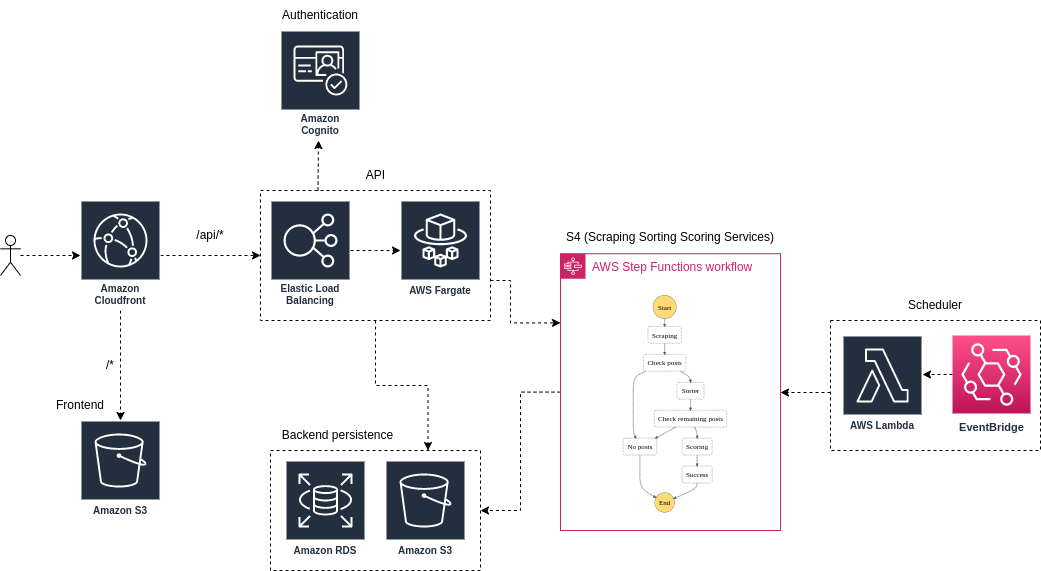
\includegraphics[width=13cm]{sezioni/images/overview.png}
    \centering
    \caption{Visione d'insieme del sistema}
\end{figure}

\subsection{Descrizione generale}
Il Backend della piattaforma sfrutta un'architettura a microservizi, i quali comunicano fra di loro secondo regole predefinite.
Le varie parti sono fra di loro indipendenti e i dati da esse prodotti persistono in RDS o bucket S3, a seconda della lora natura.
Il lavoro di analisi e progettazione ha permesso di individuare i seguenti servizi:
\begin{itemize}
    \item \textbf{API Service}: ha il compito di far interfacciare il Frontend con il resto del sistema, in particolare fornisce
    delle API RESTful che consentono l'ottenimento dei dati dal database e in generale di gestire tutte le funzionalità rese disponibili all'utente;
    \item \textbf{Scraping Service}: sfruttando apposite tecniche e librerie, effettua operazioni di scraping da Instagram al fine di ottenere dati che
    saranno successivamente processati dagli altri servizi;
    \item \textbf{Sorting Service}: effettua un preprocessing sui dati ottenuti dallo scraping, scartando eventuali dati non conformi e che comporterebbero
    uno spreco di risorse nelle fasi successive di analisi;
    \item \textbf{Scoring Service}: esegue analisi approfondite su dati testuali e multimediali, producendo una valutazione secondo alcune specifiche.
\end{itemize}

